\section{Results}

\subsection{Estimating traits via PROSPECT inversion}

\begin{figure}
  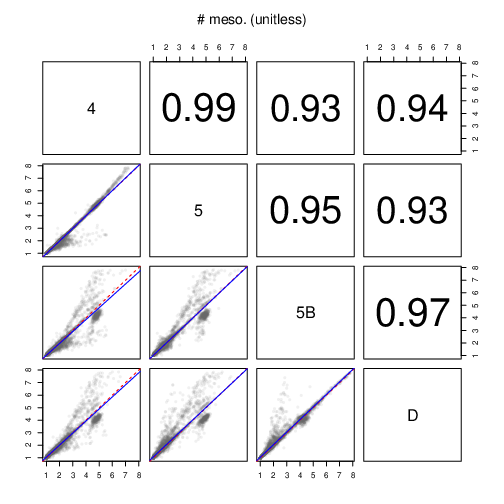
\includegraphics[width=\textwidth]{{figures/prospect_pairs_N}.png}
  \caption{\
    Inter-version comparison of estimates of number of leaf mesophyll layers.
  }\label{fig:prospect_pairs_N}
\end{figure}

\begin{figure}
  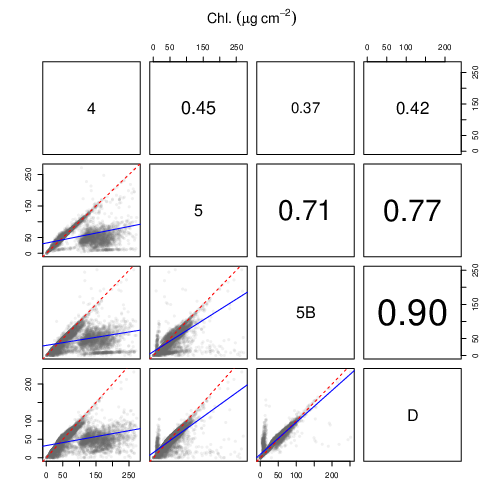
\includegraphics[width=\textwidth]{{figures/prospect_pairs_Cab}.png}
  \caption{\
    Inter-version comparison of estimates of number of total leaf chlorophyll content.
  }\label{fig:prospect_pairs_Cab}
\end{figure}

\begin{figure}
  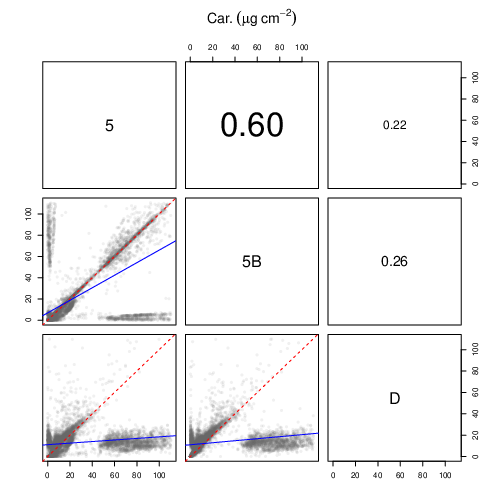
\includegraphics[width=\textwidth]{{figures/prospect_pairs_Car}.png}
  \caption{\
    Inter-version comparison of estimates of number of total leaf carotenoid content.
  }\label{fig:prospect_pairs_Car}
\end{figure}

\begin{figure}
  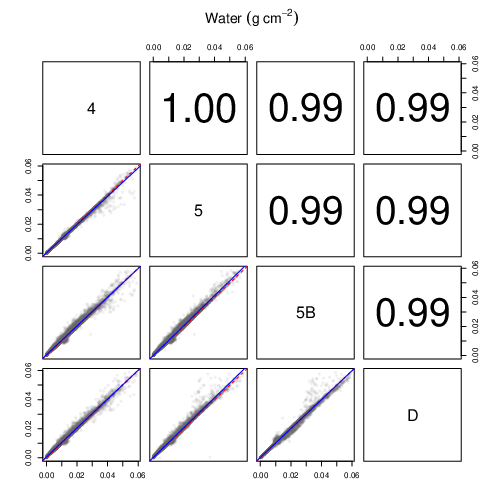
\includegraphics[width=\textwidth]{{figures/prospect_pairs_Cw}.png}
  \caption{\
    Inter-version comparison of estimates of number of total leaf water content.
  }\label{fig:prospect_pairs_Cw}
\end{figure}

\begin{figure}
  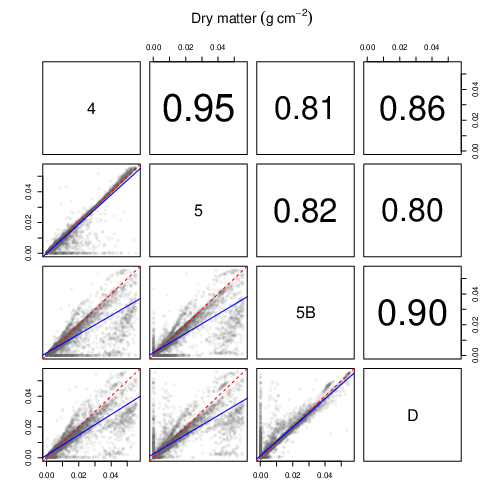
\includegraphics[width=\textwidth]{{figures/prospect_pairs_Cm}.png}
  \caption{\
    Inter-version comparison of estimates of number of total leaf dry matter content.
  }\label{fig:prospect_pairs_Cm}
\end{figure}

%TODO: Find a more concise way to represent these results

The extent of agreement on trait estimates between different versions of PROSPECT was strongly trait-dependent.
The most consistent inversion estimates were for leaf water content (Figure~\ref{fig:prospect_pairs_Cw}), which has a deep, wide-ranging, physically-based absorption coefficient that has not changed over the recent history of PROSPECT development~\cite{feret2008_prospect,feret2017_prospectd}.
Retrievals of the effective number of leaf mesophyll layers (Figure~\ref{fig:prospect_pairs_N}) and leaf dry matter content (Figure~\ref{fig:prospect_pairs_Cm}) were slightly less but still highly consistent across versions, despite changes in the refractive index and absorption features of the remaining PROSPECT parameters.
The ability of more recent versions of PROSPECT to differentiate between different types of pigments resulted in significant differences in pigment estimates between PROSPECT versions.
For chlorophyll content, the general trend is that the addition of additional pigments into the model (carotenoids in version 4, senescent brown pigments in 5, and anthocyanins in D) tends to reduce chlorophyll estimates, with the largest change happening between versions 4 and 5 (Figure~\ref{fig:prospect_pairs_Cab}).
The most significant across-version differences were in estimates of carotenoid concentrations, particularly between PROSPECT 5/5B and D, where the addition of anthocyanins led to significant reductions in estimates of carotenoid concentrations at the top of their range (Figure~\ref{fig:prospect_pairs_Car}).

\begin{figure}
  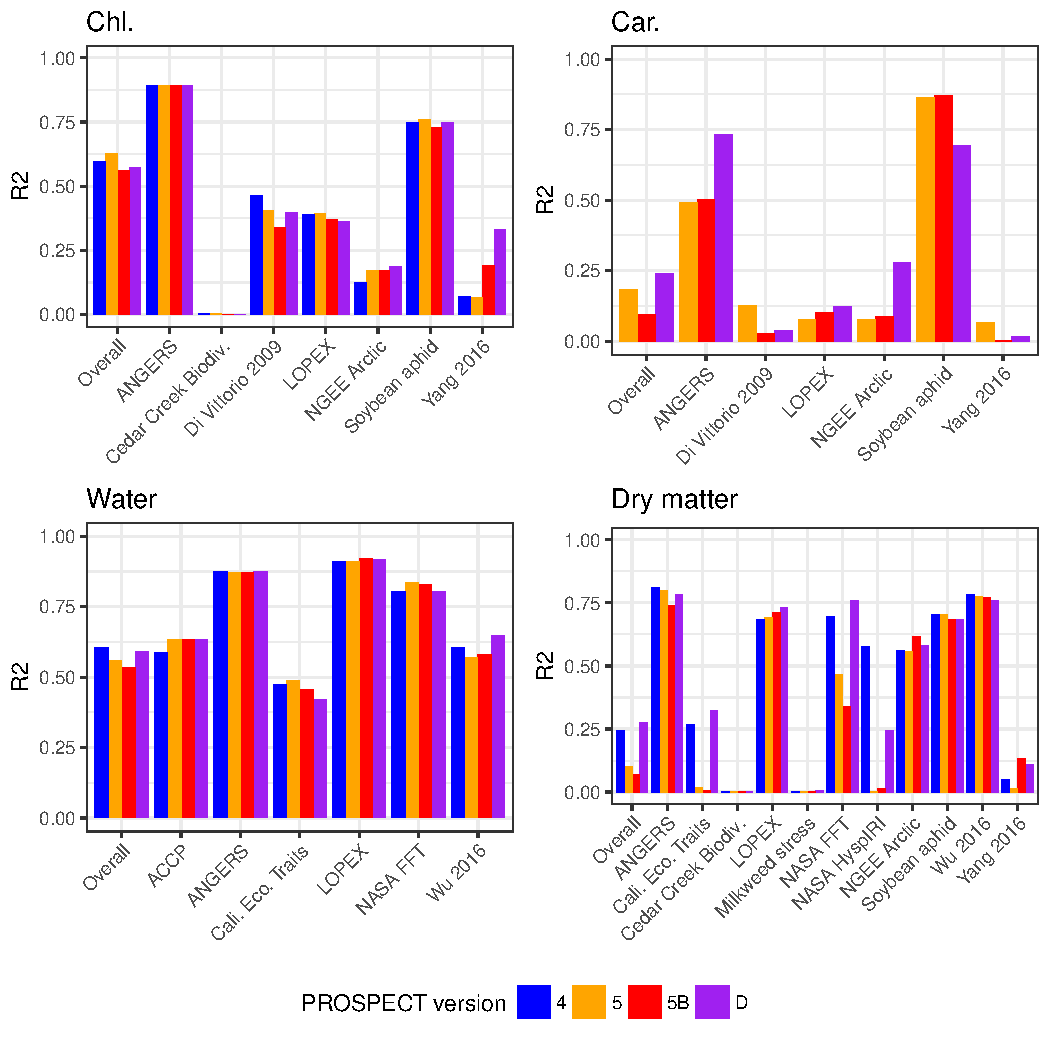
\includegraphics[width=\textwidth]{{figures/project_validation_summary}.pdf}
  \caption{\
    Validation of PROSPECT against observed trait values, by project and PROSPECT version
  }\label{fig:project_validation_summary}
\end{figure}

Across most projects and traits, the four different PROSPECT versions performed similarly in terms of their ability to retrieve traits (Figure~\ref{fig:project_validation_summary}).
For all versions of PROSPECT, leaf water content was consistently the most accurate trait retrieved, while retrievals of other traits were highly project-specific.
For several projects spanning a large range of species (Cali.\ Eco.\ Traits, NASA FFT, and NASA HyspIRI), moving from chlorophyll as the only pigment (PROSPECT 4) to chlorophyll and carotenoids (PROSPECT 5/5B) drastically reduced inversion accuracy of dry matter contents, but this accuracy was restored by the further addition of anthocyanins and modification of the refractive index in PROSPECT D (Figure~\ref{fig:project_validation_summary})
Inversion accuracy also varied significantly by project, which can largely be explained by differences in the species sampled across different projects (Supplementary Figures~\ref{fig:error_speciesbyproj_Cab}-\ref{fig:error_speciesbyproj_Cm}).
Because PROSPECT-D also retrieves anthocyanin content and generally performed as well or better than other versions, it was the version selected for subsequent analyses.
A more detailed validation for PROSPECT-D is shown in Figure~\ref{fig:prospect_D_validation}.

%TODO: More here?

\begin{figure}
  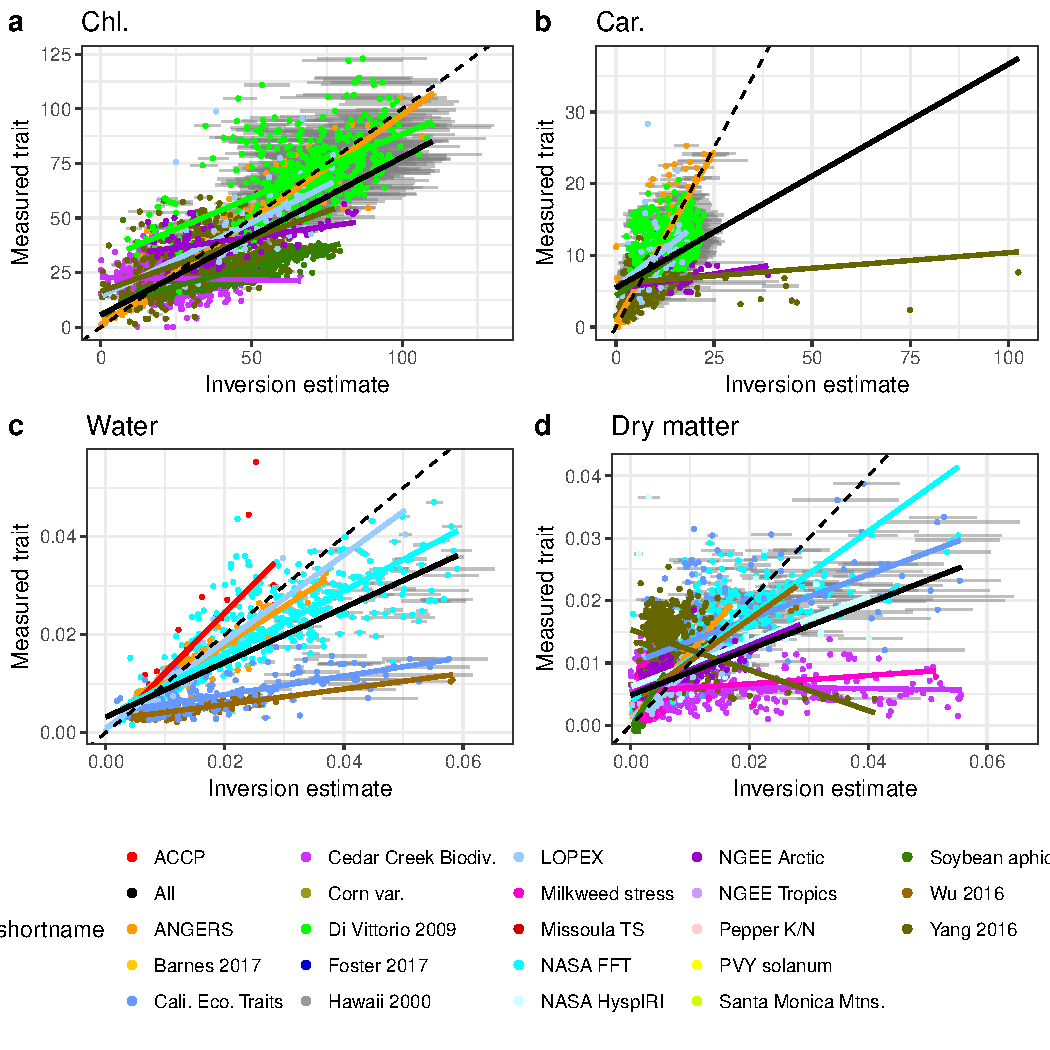
\includegraphics[width=\textwidth]{{figures/prospect_D_validation}.pdf}
  \caption{\
    Validation of PROSPECT-D against observed trait values.
    Grey lines indicate 95\% confidence intervals around trait estimates.
    Solid, colored lines are least-squares regressions fit to the data by project.
    The solid black line is a regression fit to all of the data all at once.
    The dashed black line is a 1 to 1 fit.
  }\label{fig:prospect_D_validation}
\end{figure}

\subsection{Drivers of variability in leaf optical traits}

\begin{figure}
  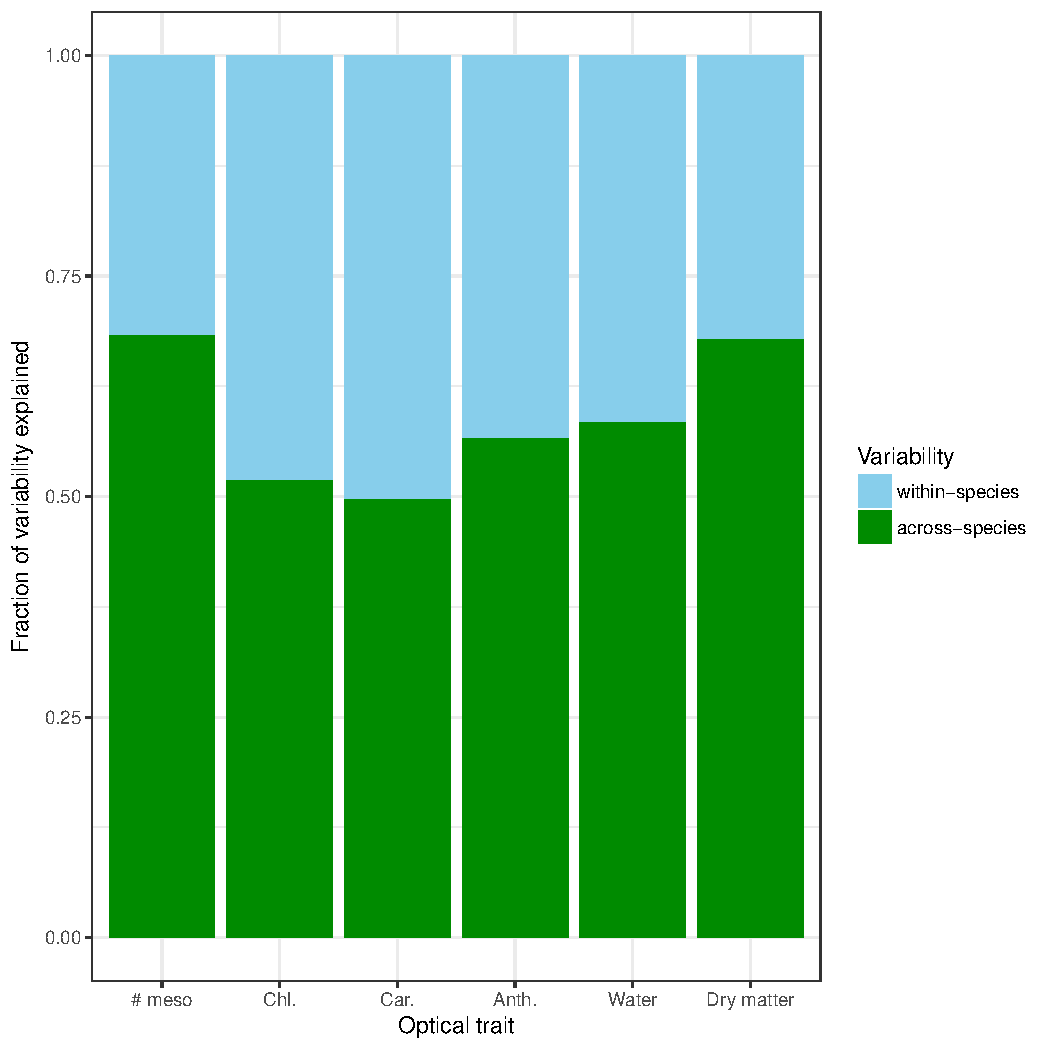
\includegraphics[width=\textwidth]{{figures/within_vs_across}.pdf}
  \caption{\
    Fraction of variance in each optical trait explained by species identity,
    based on analysis of variance on least-squares linear regression.
  }\label{fig:within_vs_across}
\end{figure}

\begin{figure}
  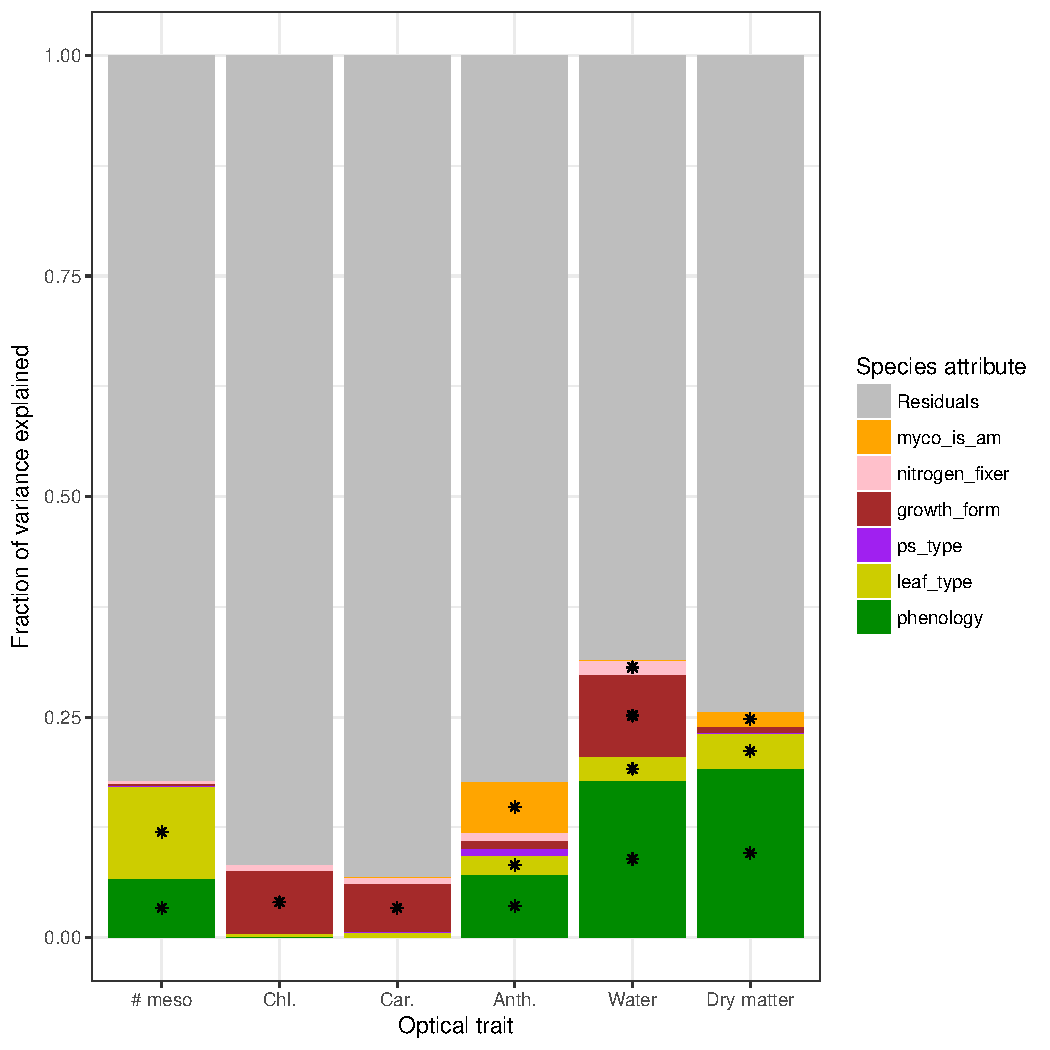
\includegraphics[width=\textwidth]{{figures/across_species_anova}.pdf}
  \caption{\
    Fraction of across-species variance in each optical trait (i.e.~species means) explained by species attributes,
    based on analysis of variance on least-squares linear regression.
    A star (*) indicates attribute effects significant at the 90\% confidence interval.
  }\label{fig:across_species_anova}
\end{figure}

Across all optical traits, roughly half of variability was explained by species identity (Figure~\ref{fig:within_vs_across}).
The variance across species means was largely ideosyncratic to species, with only up to 25\% of variance explainable by species attributes (Figure~\ref{fig:across_species_anova}).
The most important explanatory attribute was leaf phenology (deciduous vs.~evergreen), with occassional significant effects for leaf type (broad vs.~needle), growth form (woody vs.~herbaceous), and mycorrhizal association (arbuscular or non-arbuscular). 

\begin{figure}
  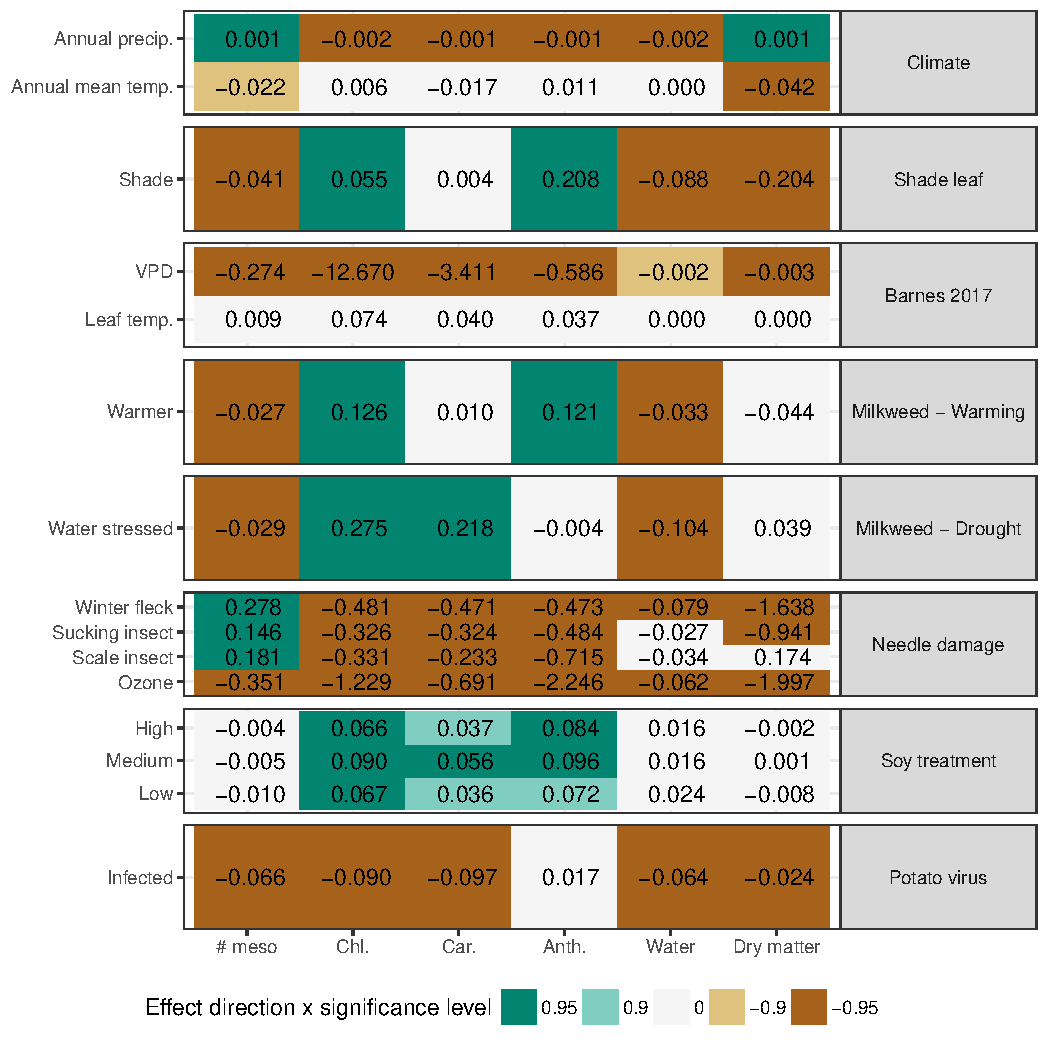
\includegraphics[width=\textwidth]{{figures/treatment_summary}.pdf}
  \caption{\
    Fixed effects of different sources of intraspecific variability on traits estimated from PROSPECT inversion.
    Each value is the perecnt fixed effect on the corresponding trait as estimated from a linear fixed-effects model.
    Color brightness indicates degree of statistical significance (90 or 95\% confidence level), and color hues indicate effect direction (positive or negative).
  }\label{fig:treatment_summary}
\end{figure}

Leaf optical traits responded significantly to a range of natural and experimental stressors (Figure~\ref{fig:treatment_summary}).
Intraspecific variability in optical traits was weakly but, in some cases, significantly related to climate, with the strongest effects being declines in leaf number of mesophyll layers and dry matter content with increasing temperature.
Based on leaf reflectance measurements of \textit{Populus deltoides} (eastern cottonwood) at the University of Arizona by Barnes et al.~(2017), \nocite{barnes_2017_beyond}
seasonal variations in leaf and air temperature had statistically significant but relatively small impacts on pigment concentrations.
Warming and drought experiments on \textit{Asclepias syriaca} (common milkweed) had strong and statistically significant effects on almost all optical traits, with both treatments leading to significant decreases in leaf water content and effective number of mesophyll layers and increases in pigments and dry matter content concentrations.
In two independent studies, optical traits also responded significantly to chemical (ozone, winter fleck) and biotic (insects, viruses) stressors---all of these stressors significantly reduced concentrations of pigments, and typically also reduced water and dry matter contents, with ozone damage having the most significant effect.
On the other hand, treatment of \textit{Glycine max} (soybean) with aphids resulted in a small but significant increase in pigment concentrations, with the strongest effect observed at medium-level treatment.
Finally, across the projects and species for which data were available for both sunlit and shaded leaves, shaded leaves had higher chlorophyll and anthocyanin concentrations and lower number of mesophyll layers and water and dry matter contents.

\begin{figure}
  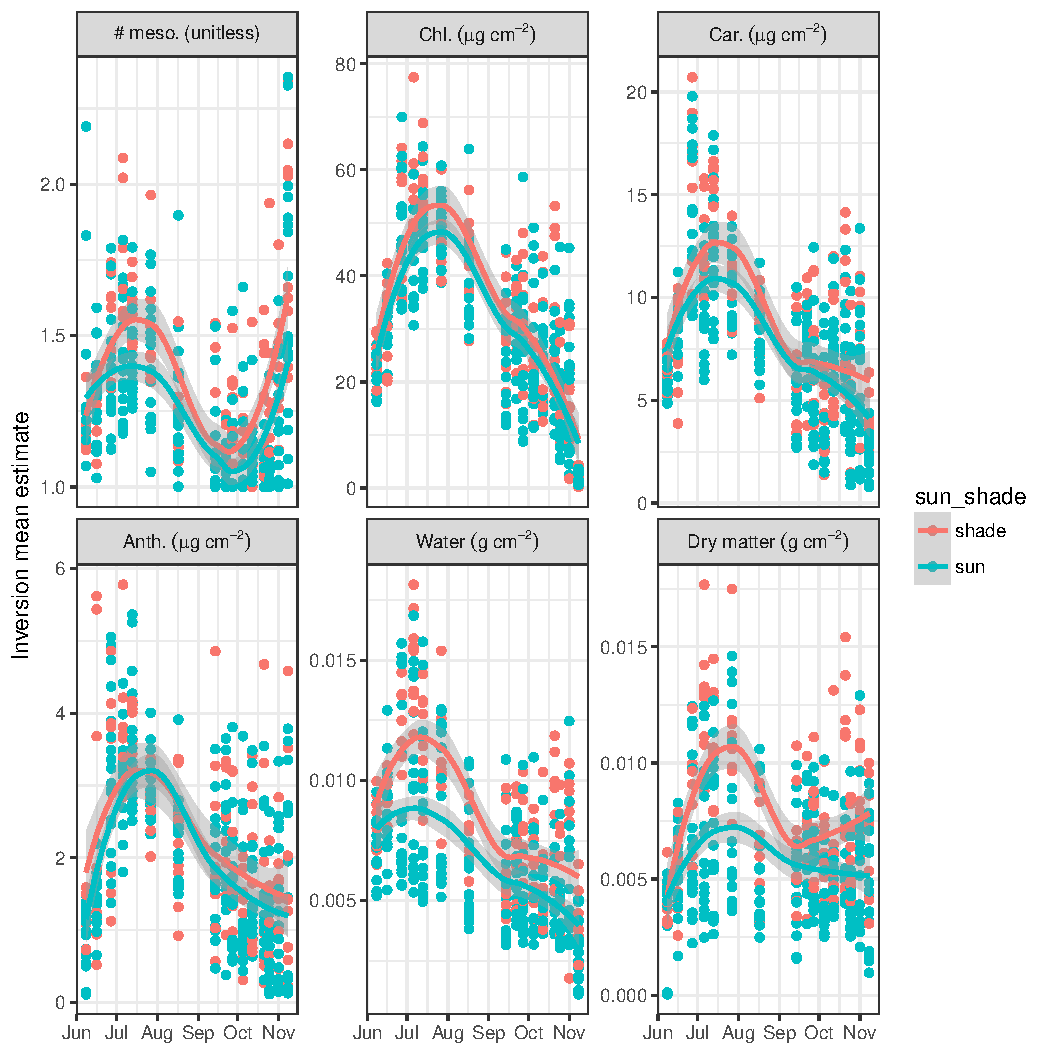
\includegraphics[width=\textwidth]{{figures/trait_phenology}.pdf}
  \caption{\
    Optical trait estimates through a season for Quercus rubra (red oak) at Martha's Vineyard, MA by Yang et al.~(2016).
    Colors indicate sunlit vs.~shaded leaves.
    Line is a LOESS best fit with shaded standard error.
  }\label{fig:trait_phenology}
  \nocite{yang_2016_seasonal}
\end{figure}

Where such measurements were available, leaf optical traits exhibited a strong phenological signal (Figure~\ref{fig:trait_phenology}).
All optical traits showed a peak in late July / early August, followed by a decline into the fall.
However, the effective number of leaf mesophyll layers, and to a lesser extent, leaf dry matter content in sunlit leaves increased in the late fall. 
With the exception of anthocyanin content, traits for sunlit leaves were higher and experienced a greater seasonal variability than shaded leaves.

\subsection{Correlations of optical traits with other traits}

\begin{figure}
  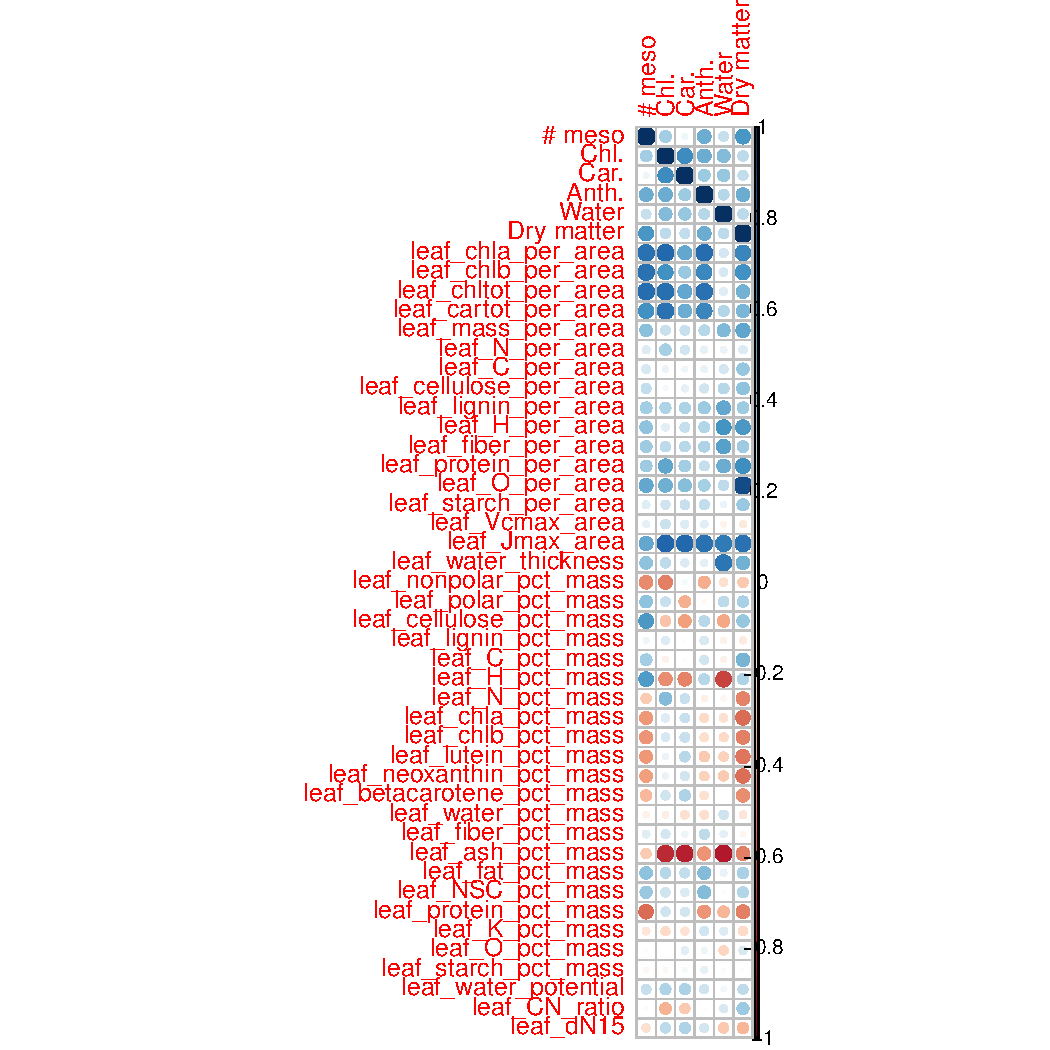
\includegraphics[width=\textwidth]{{figures/trait_correlations_all}.pdf}
  \caption{\
    Correlations of optical trait estimates with direct trait measurements, by all observations.
  }\label{fig:trait_correlations_all}
\end{figure}

Optical traits estimated by PROSPECT were generally mutually positively correlated with each other.
The strongest pairwise correlations were of dry matter content with the effective number of leaf mesophyll layers, and of chlorophyll and carotenoid contents.

With the exception of leaf water content, all optical traits were strongly positively correlated with direct area-based measurements of pigments, and less strongly correlated with a number of area-based traits.
Leaf chlorophyll content exhibited moderate positive correlations with nitrogen, protein, and oxygen concentrations.
Leaf carotenoid and anthocyanin contents exhibited weak positive correlations with lignin, fiber, protein, hydrogen, and oxygen concentrations.
Leaf water content was strongly positively correlated with lignin, fiber, protein, and hydrogen concentrations, though surprisingly not oxygen concentration.
Finally, leaf dry matter content was positively correlated with all area-based traits available, with the weakest correlation for nitrogen and the strongest correlations for oxygen, hydrogen, and protein.
All optical traits had negligible correlations with Vcmax, but very strong positive correlations with Jmax.
Chlorophyll, carotenoids, and dry matter were positively correlated with leaf water potential.
Pigments were weakly positively correlated, and remaining traits weakly negatively correlated, with leaf $\Delta N_{15}$ concentration.
Patterns of species means were generally similar to patterns observed within species (Figure~\ref{fig:trait_correlations_species}).

% TODO: Mass traits?

%On a mass basis, leaf number of mesophyll layers and dry matter contents were negatively correlated with direct pigment measurements and protein contents and weakly positively correlated with cellulose, hydrogen, fat, and non-structural carbohydrates.
%Pigments exhibited strong
